\documentclass{beamer}

\mode<presentation> {
\usetheme{AnnArbor}
}

\usepackage{graphicx}
\graphicspath{{./figures/}}
\usepackage{caption}
\usepackage{subcaption}
\usepackage{hyperref}
\hypersetup{colorlinks=true}
\usepackage{amsmath}
\usepackage{amsthm}
\usepackage{multirow}
\usepackage{siunitx}
\usepackage{biblatex}
\usepackage{algorithm}
\usepackage{algpseudocode}
\addbibresource{bibliography.bib}

\AtEveryBibitem{
    \clearfield{doi}
    \clearfield{isbn}
    \clearfield{issn}
    \clearlist{language}
    \clearfield{note}
    \clearfield{url}
    \clearfield{urlyear}
}

\setbeamertemplate{caption}[numbered]

\newtheorem{assumption}{Assumption}[section]
\newtheorem{proposition}{Proposition}
\newtheorem{remark}{Remark}[section]
\def\C{\mathbb C}
\def\E{\mathbb E}
\def\I{\mathbb I}
\def\P{\mathbb P}
\def\R{\mathbb R}
\def\RV{\text{RV}}
\def\Z{{\mathbb Z}}
\def\FPR{\text{FPR}}
\def\TPR{\text{TPR}}
\def\sign{{\rm sign}}
\def\ind{\perp\!\!\!\perp}
\def\seqSet{\mathcal{C}_{\alpha}}
\def\series{\xi}
\newcommand\Fi[1]{F_{#1}^{\leftarrow}}
\newcommand{\multiplier}[2]{\kappa_{#1}(#2)}
\newcommand{\mmultiplier}[4]{\kappa_{#1, #2}(#3, #4)}
\newcommand{\normConst}[3]{\eta_{#1}({#2}, {#3})}
\newcommand{\pred}[1]{\hat{Y}_{t + h}^{\text{(#1)}}}
\newcommand{\AROptPred}[3]{\hat{Y}_{#1 + #2}(#3)}
\newcommand{\approxAROptPred}[3]{\hat{Y}_{#1 + #2}(\hat{#3})}
\DeclareMathOperator*{\argmin}{arg\,min}
\DeclareMathOperator*{\argmax}{arg\,max}

\title[Optimal Prediction of Extreme Events]{Optimal Prediction of Extreme Events \\ with Applications to Solar Flare Forecasting}

\author{Victor Verma, Stilian Stoev, Yang Chen}
\institute[]
{
Department of Statistics \\
University of Michigan
}
\date[7/18/24]{7/18/24}

\begin{document}

\begin{frame}
    \titlepage
\end{frame}

\begin{frame}{Outline}
   \tableofcontents
\end{frame}

\section{Introduction}

\begin{frame}{Solar Flares}
    \begin{itemize}
        \item Solar flares: sudden, massive eruptions of electromagnetic radiation from the Sun's atmosphere
        \item Adverse effects of solar flares: 
        \begin{itemize}
            \item Radio blackouts
            \item Coronal mass ejection (CME) $\rightarrow$ electromagnetic pulse $\rightarrow$ electrical blackouts
            \item Solar energetic particle event (SEP) $\rightarrow$ irradiation of astronauts
        \end{itemize}
        \item Some notable incidents:
        \begin{itemize}
            \item 1989: Quebec's electrical grid was shut down for several hours
            \item 2022: Dozens of Starlink satellites were destroyed
        \end{itemize}
    \end{itemize}
\end{frame}

\begin{frame}{The X-Ray Flux}
    \begin{figure}
        \centering
        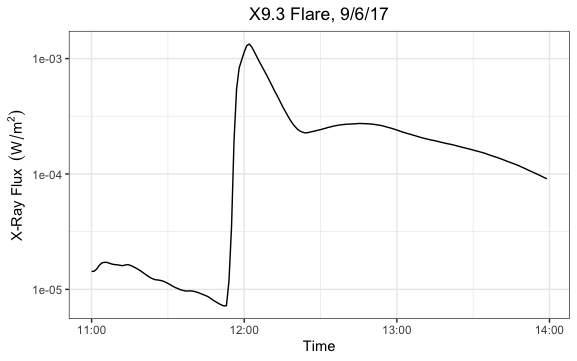
\includegraphics[scale=0.5]{flare_flux_example.png}
        \caption{The X-ray flux around the time of a strong flare.}
        \label{fig:flare_flux_example}
    \end{figure}
\end{frame}

\begin{frame}{The X-Ray Flux}
    \begin{figure}
        \centering
        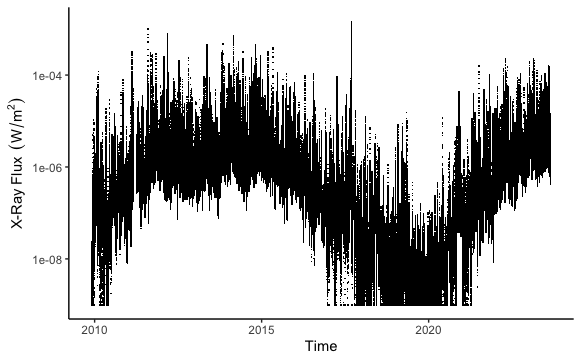
\includegraphics[scale=0.5]{flux_plot.png}
        \caption{The X-ray flux time series.}
        \label{fig:flux_plot}
    \end{figure}
\end{frame}

\begin{frame}{Flare Strength}
    Flare strength is determined by the peak (soft) X-ray flux.
    \begin{table}
        \centering
        \begin{tabular}{|c|c|}
            \hline
            Flare Class & X-Ray Flux Threshold ($\text{W} / \text{m}^2$) \\
            \hline
            A & $10^{-8}$ \\
            B & $10^{-7}$ \\
            C & $10^{-6}$ \\
            M & $10^{-5}$ \\
            X & $10^{-4}$ \\
            \hline
        \end{tabular}
        \caption{X-ray flux thresholds for the different flare classes}
        \label{tab:flare_classes}
    \end{table}

    \textbf{
        Goal:
        \begin{center}
            Forecast flares by predicting whether the flux will exceed a threshold
        \end{center}
    }
\end{frame}

\begin{frame}{Existing Work}
    Example: Deep Flare Net \cite{nishizuka2018deep, nishizuka2021oper}
    \begin{itemize}
        \item Predicts whether strong flare will occur in next 24 hours
        \item For M+ class flares, non-operational TSS = 0.8, operational = 0.24
    \end{itemize}    
    The flare forecasting problem has not been solved:
    \begin{itemize}
        \item Forecasting methods were compared in operational setting in \cite{leka2019acomII, leka2019acomIII}
        \item Goal: predict if C+ class or M+ class flare will occur in next 24 hours
        \item For both, no method attained a TSS over 0.5.
        \item ML-based methods tended to perform worse
    \end{itemize}
\end{frame}

\section{Foundations of Optimal Extreme Event Prediction}

\begin{frame}{The Statistical Problem}
    Let $Y$ be a random variable with CDF $F_Y$ and quantile function $F_Y^{-1}$. Let $X$ be a random vector in $\R^d$.

    \medskip
    
    \textbf{
    The flare forecasting problem is an instance of this general problem:
    \begin{center}
        Predict whether $Y > F_Y^{-1}(p)$ using $g(X)$ for some suitable $g$.
    \end{center}
    }
    Example:
    \begin{itemize}
        \item $Y$: flux at time $t + h$
        \item $X$: vector of fluxes at times $t, \ldots, t - \ell$
    \end{itemize}

    \medskip
    
    Assume that $F_Y$ is continuous at $F_Y^{-1}(p)$. Then $\P(Y > F_Y^{-1}(p)) = 1 - p$.
\end{frame}

\begin{frame}{Calibration and Optimality of Predictors}
    Indicators can be used to represent both the predictand and a predictor:
    \[
    \I(Y > \Fi{Y}(p)), \ \I(g(X) > \tau)
    \]
    \begin{definition}
        \begin{itemize}
            \item $\I(g(X) > \tau)$ is calibrated if $\P(g(X) > \tau) = 1 - p$
            \item $\I(g(X) > \tau)$ is optimal if it is calibrated and for any other calibrated predictor $\I(k(X) > \rho)$,
            \begin{equation}\label{eq:optimality_cond}
                \P(Y > \Fi{Y}(p) \mid g(X) > \tau) \ge \P(Y > \Fi{Y}(p) \mid k(X) > \rho)
            \end{equation}
        \end{itemize}
    \end{definition}
    We call probabilities like those in \eqref{eq:optimality_cond} precisions.
\end{frame}

\begin{frame}{Optimal Predictors in the General Case}
    \begin{itemize}
        \item Let $X$ and $Y$ have a joint density $f$ with respect to the Lebesgue measure on $\R^d \times \mathbb{R}$.
        \item Let $f_0$ be the conditional density of $X$ given that $Y \le \Fi{Y}(p)$
        \item Let $f_1$ be the conditional density of $X$ given that $Y > \Fi{Y}(p)$
    \end{itemize}
    Then
    \[
    f_0(x) = \frac{1}{p}\int_{-\infty}^{\Fi{Y}(p)} f(x, y)\,dy, \
    f_1(x) = \frac{1}{1 - p}\int_{\Fi{Y}(p)}^{\infty} f(x, y)\,dy
    \]
    \begin{theorem}
        Let $r(x) = f_1(x) / f_0(x)$. Suppose that $F_{r(X)}$ is continuous at $\Fi{r(X)}(p)$. Then $\I(r(X) > \Fi{r(X)}(p))$ is an optimal predictor of $\I(Y > \Fi{Y}(p))$.
    \end{theorem}
\end{frame}

\begin{frame}{Optimal Predictors in Special Cases}
    \begin{theorem}
        Let $X \in \R^d$ and $\epsilon \in \R$, with $X \ind \epsilon$, and let $\sigma$ be a function that is positive on the range of $X$. Suppose that $Y = \mu(X) + \sigma(X)\epsilon$. Then an optimal predictor of $\I(Y > \Fi{Y}(p))$ is $\I(g(X) > \Fi{g(X)}(p))$, where
        \[
        g(X) = \frac{\mu(X) - \Fi{Y}(p)}{\sigma(X)},
        \]
        assuming that $F_{g(X)}$ is continuous at $\Fi{g(X)}(p)$.
    \end{theorem}
    \begin{corollary}
        When $\sigma(X)$ is constant, and $F_{\mu(X)}$ is continuous at $\Fi{\mu(X)}(p)$, then an optimal predictor is
        \[
        \I(\mu(X) > \Fi{\mu(X)}(p)).
        \]
    \end{corollary}
\end{frame}

\section{Optimal Extreme Event Prediction in Linear Time Series}

\begin{frame}{MA($\infty$) Models}
    Consider the moving average (MA) model of order $\infty$
    \begin{equation}\label{eq:ma_infty_mod}
        Y_t = \sum_{j = 0}^{\infty} a_j\epsilon_{t - j}.
    \end{equation}
    Assume that the series in \eqref{eq:ma_infty_mod} converges absolutely almost surely. An example of conditions that ensure this:
    \begin{itemize}
        \item $\sum_{j = 0}^{\infty} |a_j| < \infty$
        \item $\epsilon_t$'s are uncorrelated with mean 0 and variance $\sigma^2$
    \end{itemize}

    \textbf{
        \begin{center}
            Goal: Predict whether $Y_{t + h} > \Fi{Y}(p)$ using $Y_s$ for $s \le t$
        \end{center}
    }
\end{frame}

\begin{frame}{An Optimal Predictor for MA($\infty$) Models}
    We have
    \[
    Y_{t + h}    
    = \sum_{j = 0}^{\infty} a_{j + h}\epsilon_{t - j} + \sum_{j = 0}^{h - 1} a_j\epsilon_{t + h - j}.
    \]
    $\{Y_t\}$ is invertible if there exists $\{b_j\}_{j = 0}^{\infty} \subset \R$ such that for all $t$, almost surely,
    \[
    \epsilon_t = \sum_{j = 0}^{\infty} b_j Y_{t - j}.
    \]

    \begin{theorem}
        Suppose $\{Y_t\}$ is invertible. Then for every $h \ge 1$, the optimal predictor of $Y_{t + h}$ based on $Y_s$, $s \le t$, is
        \[
        \pred{opt} := \sum_{j = 0}^{\infty} a_{j + h}\epsilon_{t - j}.
        \]
    \end{theorem}
\end{frame}

\begin{frame}{Approximating the Optimal Predictor}
    $\pred{opt}$ can be written as
    \[
    \sum_{j = 0}^{\infty} \sum_{k = 0}^{\infty} a_{j + h}b_k Y_{t - j - k} = \sum_{r = 0}^{\infty}\left[\sum_{s = 0}^r a_{s + h}b_{r - s}\right]Y_{t - r}
    =: \sum_{r = 0}^{\infty} c_r Y_{t - r},
    \]
    If the $\ell \ge 1$ most recent observations, i.e., $Y_t, \ldots, Y_{t - \ell + 1}$, are available at time $t$, then we approximate $\pred{opt}$ by
    \[
    \widehat{Y}_{t + h}^{(\ell)} = \sum_{r = 0}^{\ell - 1} c_r Y_{t - r},
    \]
    where $c_r = \sum_{s = 0}^r a_{s + h}b_{r - s}$.
\end{frame}

\begin{frame}{A Special Case: AR($d$) Models}
    Consider the autoregressive (AR) model of order $d$
    \begin{equation*}
        Y_t = \sum_{j = 1}^d \phi_j Y_{t - j} + \epsilon_t, \ t \in \Z.
    \end{equation*}
    Assume that
    \begin{itemize}
        \item the $\epsilon_t$'s are iid
        \item for all $t$, $\epsilon_t$ is independent of $Y_{t - 1}, Y_{t - 2}, \ldots$
        \item $\{Y_t\}$ is stationary and causal
    \end{itemize}

    \medskip

    \textbf{
        \begin{center}
            Goal: Predict whether $Y_{t + h} > \Fi{Y}(p)$ using $Y_s$ for $s \le t$
        \end{center}
    }
\end{frame}

\begin{frame}{An Optimal Predictor for AR($d$) Models}
    Observation: for all $h \ge 1$,
    \[
    Y_{t + h} = \phi(h)^{\top}Y_{t:(t - d + 1)} + \eta_{t + h},
    \]
    where
    \begin{itemize}
        \item $\phi(h) := \Phi^h e_1$, $\Phi := (\begin{matrix} \phi & e_1 & \cdots & e_{d - 1} \end{matrix}) \in \R^{d \times d}$
        \item $\eta_{t + h} \ind Y_t, \ldots, Y_{t - d + 1}$
    \end{itemize}
    \begin{theorem}
        The optimal predictor of $\I(Y_{t + h} > \Fi{Y}(p))$ via $Y_{t:(t - d + 1)}$ is $\I(\AROptPred{t}{h}{\phi} > F_{\AROptPred{t}{h}{\phi}}^{\leftarrow}(p))$, where
        \[
        \AROptPred{t}{h}{\phi} := \phi(h)^{\top}Y_{t:(t - d + 1)}.
        \]
    \end{theorem}    
\end{frame}

\begin{frame}{AR($d$) Prediction Methodology}
    \begin{figure}[h]
        \centering
        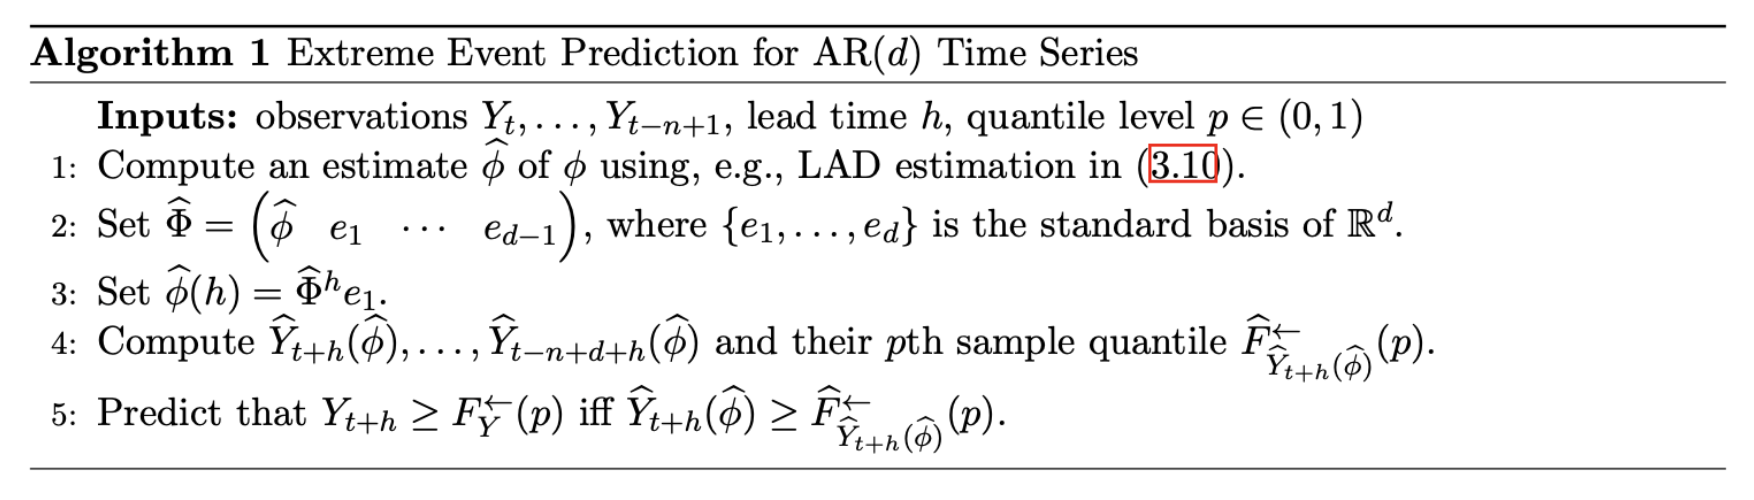
\includegraphics[scale=0.4]{figures/ar_algorithm.png}
        \label{fig:ar_algorithm}
        \end{figure}    
\end{frame}

\begin{frame}{Consistency of the Approximation}
    Let $\hat{q}$ be the $p$th sample quantile of
    \[
    \{\approxAROptPred{t}{h}{\phi}, \ldots, \approxAROptPred{t - (n - d)}{h}{\phi}\}.
    \]
    \begin{theorem}
        Suppose that $\hat{\phi} \xrightarrow{\P} \phi$ and $\hat{q} \xrightarrow{\P} q := F_{\AROptPred{t}{h}{\phi}}^{\leftarrow}(p)$.
        
        Also suppose that $\Fi{Y}(p)$ is a continuity point of $F_Y$ and that $q$ is a continuity point of $F_{\AROptPred{t}{h}{\phi}}$.
        
        Then $\I(\approxAROptPred{t}{h}{\phi} \ge \hat{q})$ is:
        
        (i) Asymptotically calibrated, i.e., as $n \to \infty$,
        \[
        \P(\approxAROptPred{t}{h}{\phi} \ge \hat{q}) \to 1 - p = \P(Y_{t + h} > \Fi{Y}(p))
        \]
        
        (ii) Asymptotically optimal, i.e., as $n \to \infty$,
        \[
        \P(Y_{t+h} \ge \Fi{Y}(p) \mid \approxAROptPred{t}{h}{\phi} \ge \hat{q}) \to \lambda_p(Y_{t + h}, \AROptPred{t}{h}{\phi})
        \]
    \end{theorem}
\end{frame}

\section{Simulations}

\begin{frame}{Simulation Setup}
    Data was generated from the AR(5) model
    \begin{equation}\label{eq:sim_ar_mod}
        Y_t = 0.3 Y_{t - 1} + 0.19 Y_{t - 2} - 0.035 Y_{t - 3} - 0.01 Y_{t - 4} + 0.0025 Y_{t - 5} + \epsilon_t,    
    \end{equation}
    with the $\epsilon_t$'s being iid $t$-distributed with one degree of freedom. The corresponding AR polynomial has roots $-3 \pm 1i$, $4 \pm 2i$, and $2$; since these roots lie outside the closed unit disk, \eqref{eq:sim_ar_mod} has a unique solution that is stationary and causal.
\end{frame}

\begin{frame}{Setup}
    \begin{itemize}
        \item Generate large time series of size $10^6$ from \eqref{eq:sim_ar_mod}.
        \item For each $p \in \{0.90, 0.95, 0.99, 0.999\}$, $\Fi{Y}(p)$ was estimated as the $p$th sample quantile of the time series.
        \item All possible linear combinations of the form $\phi^{\top}Y_{t:(t - 4)}$ were computed using the time series; $\Fi{\AROptPred{t}{h}{\phi}}(p)$ was estimated as the $p$th sample quantile of these linear combinations.
        \item Next, one hundred times, a time series of length $10^4 + 10^6$ was generated from the model in \eqref{eq:sim_ar_mod}; the first $10^4$ observations were reserved for training, and the last $10^6$ were reserved for testing.
    \end{itemize}
\end{frame}

\begin{frame}{Setup}
    For a test observation $Y_{t + 1}$, the oracle predictor predicted that $Y_{t + 1} > \Fi{Y}(p)$ iff 
    \[
    \phi^{\top}Y_{t:(t - 4)} > \Fi{\AROptPred{t}{h}{\phi}}(p).
    \]
    The predictor based on the empirical quantile estimator predicted an exceedance iff
    \[
    \widehat{\phi}^{\top}Y_{t:(t - 4)} > \widehat{F}_{\approxAROptPred{t}{h}{\phi}}^{\leftarrow}(p)),
    \]
    where $\widehat{F}_{\approxAROptPred{t}{h}{\phi}}^{\leftarrow}(p))$ was computed as the $p$th sample quantile of all linear combinations of the form $\widehat{\phi}^{\top}Y_{s:(s - 4)}$ that could be computed from the training set.
\end{frame}

\begin{frame}{Extreme Quantile Estimator}
    The predictor based on the extreme quantile estimator predicted an exceedance iff
    \[
    \widehat{\phi}^{\top}Y_{t:(t - 4)} > \widetilde{F}_{\approxAROptPred{t}{h}{\phi}}^{\leftarrow}(p)),
    \]
    where $\widetilde{F}_{\approxAROptPred{t}{h}{\phi}}^{\leftarrow}(p))$ was computed from the training set using an extreme quantile estimator.
\end{frame}

\begin{frame}{Extreme Quantile Estimator}
    The GP distribution with scale parameter $\sigma > 0$ and shape parameter $\xi$ has a distribution function that equals
    \[
    G(y) = 1 - \left(1 + \frac{\xi y}{\sigma}\right)^{-1 / \xi}.
    \]
    The Kolmogorov-Smirnov test was used to identify the value for which the GP model fit best; the value with the smallest test statistic was used. Denote this value by $\tau$, and let $p_0$ be the proportion of linear combinations less than or equal to $\tau$. The extreme quantile estimate was computed as
    \[
    \widetilde{F}_{\approxAROptPred{t}{h}{\phi}}^{\leftarrow}(p)) = \tau + \widehat{G}^{\leftarrow}\left(\frac{p - p_0}{1 - p_0}\right),
    \]
    the second term on the right being the $(p - p_0) / (1 - p_0)$ quantile of the fitted model $\widehat{G}$.
\end{frame}

\begin{frame}{Simulation Results}
    \begin{figure}[!htb]
    \centering
    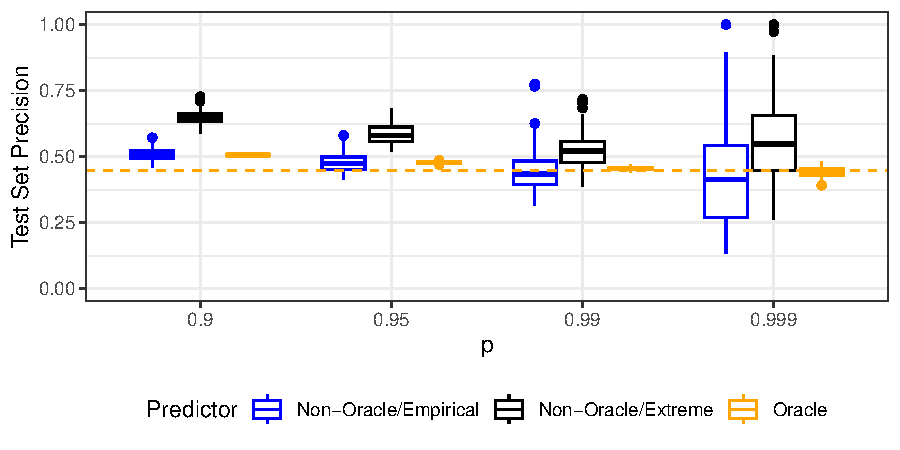
\includegraphics[width=0.7\textwidth]{figures/quantile_type_impact.pdf}
    \label{fig:quantile_type_impact}
    \end{figure}
\end{frame}

\section{Data Analysis}

\begin{frame}{Data Processing}
    Original data: minutely GOES X-ray flux data from 7/27/1998-5/11/2024.

    Processing steps:
    \begin{itemize}
        \item Retained measurements from both
        \begin{itemize}
            \item 1/1/2000-12/31/2002 ($\approx$ maximum of solar cycle 23)
            \item 9/1/2011-5/31/2014 ($\approx$ maximum of solar cycle 24)
            \item \href{https://www.swpc.noaa.gov/products/solar-cycle-progression}{SWPC Solar Cycle Progression product}\footnote{\url{https://www.swpc.noaa.gov/products/solar-cycle-progression}} was used to identify the maxima.
        \end{itemize}
        \item Took the maximum flux over each hour of the day; produced a time series of length 50,400.
        \item Used linear interpolation to impute a few missing values ($< 1\%$ of values).
    \end{itemize}
\end{frame}

\begin{frame}{Identifying Solar Cycle Maxima}
    \begin{figure}[h]
    \centering
    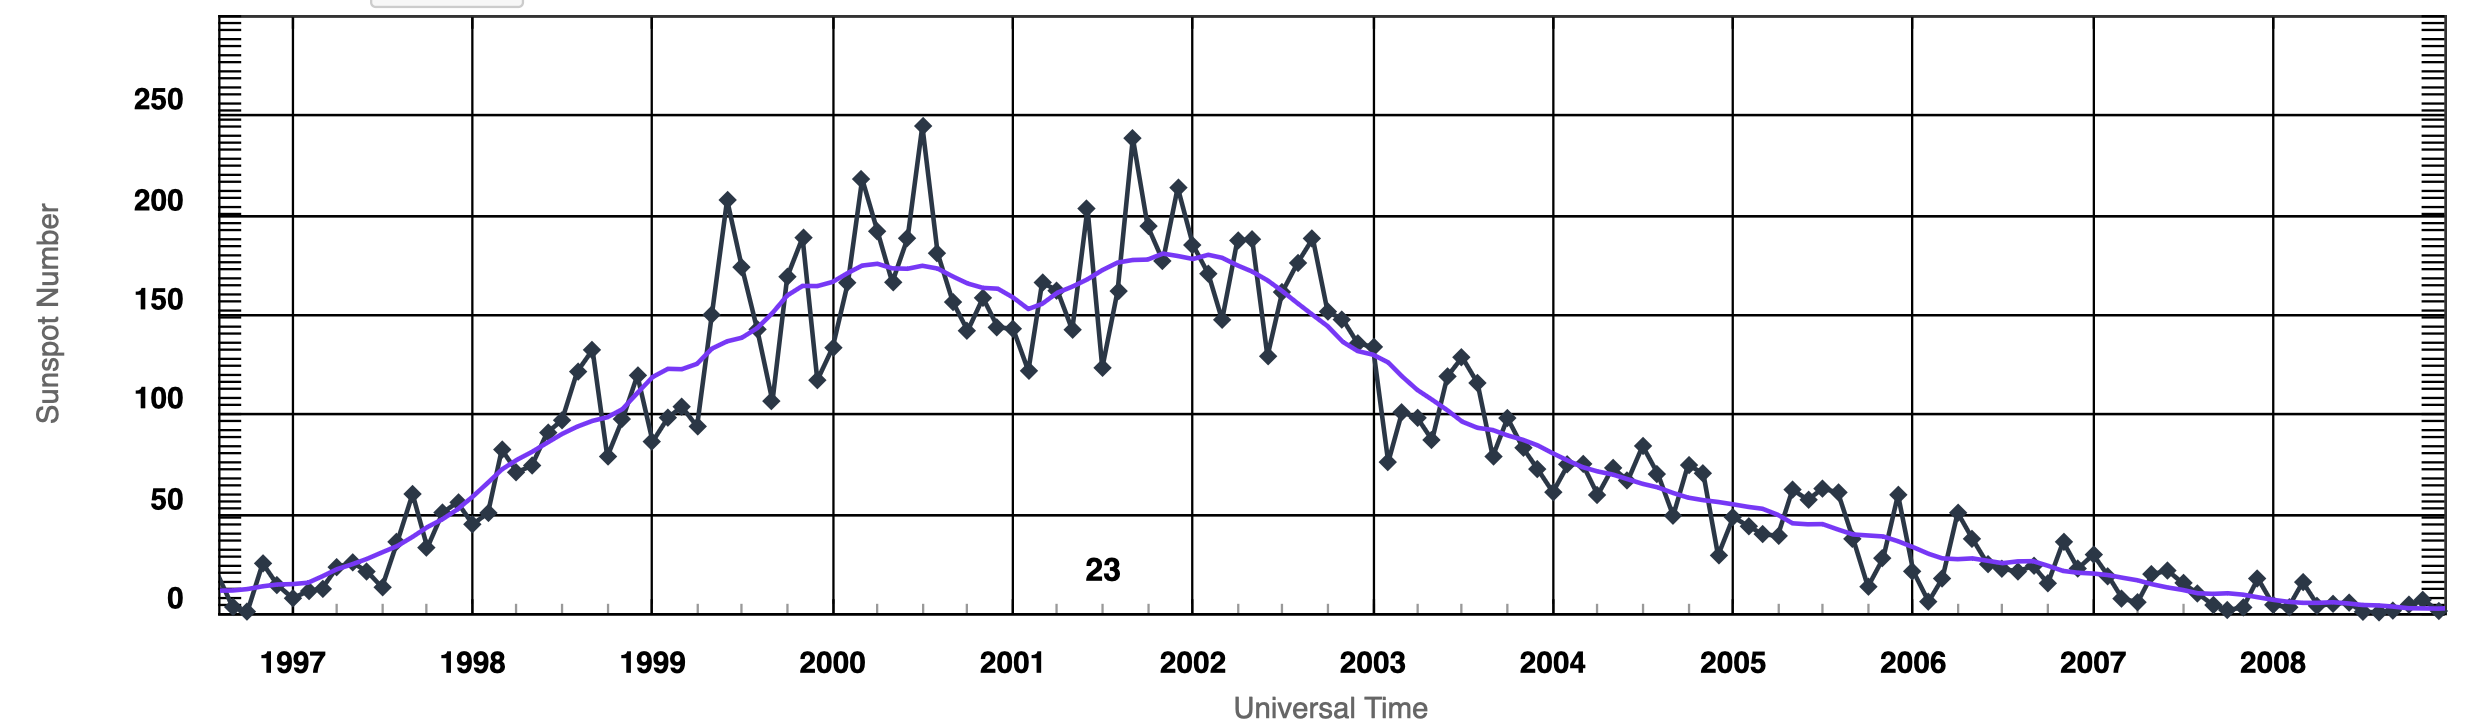
\includegraphics[scale=0.25]{figures/solar_cycle_23.png}
    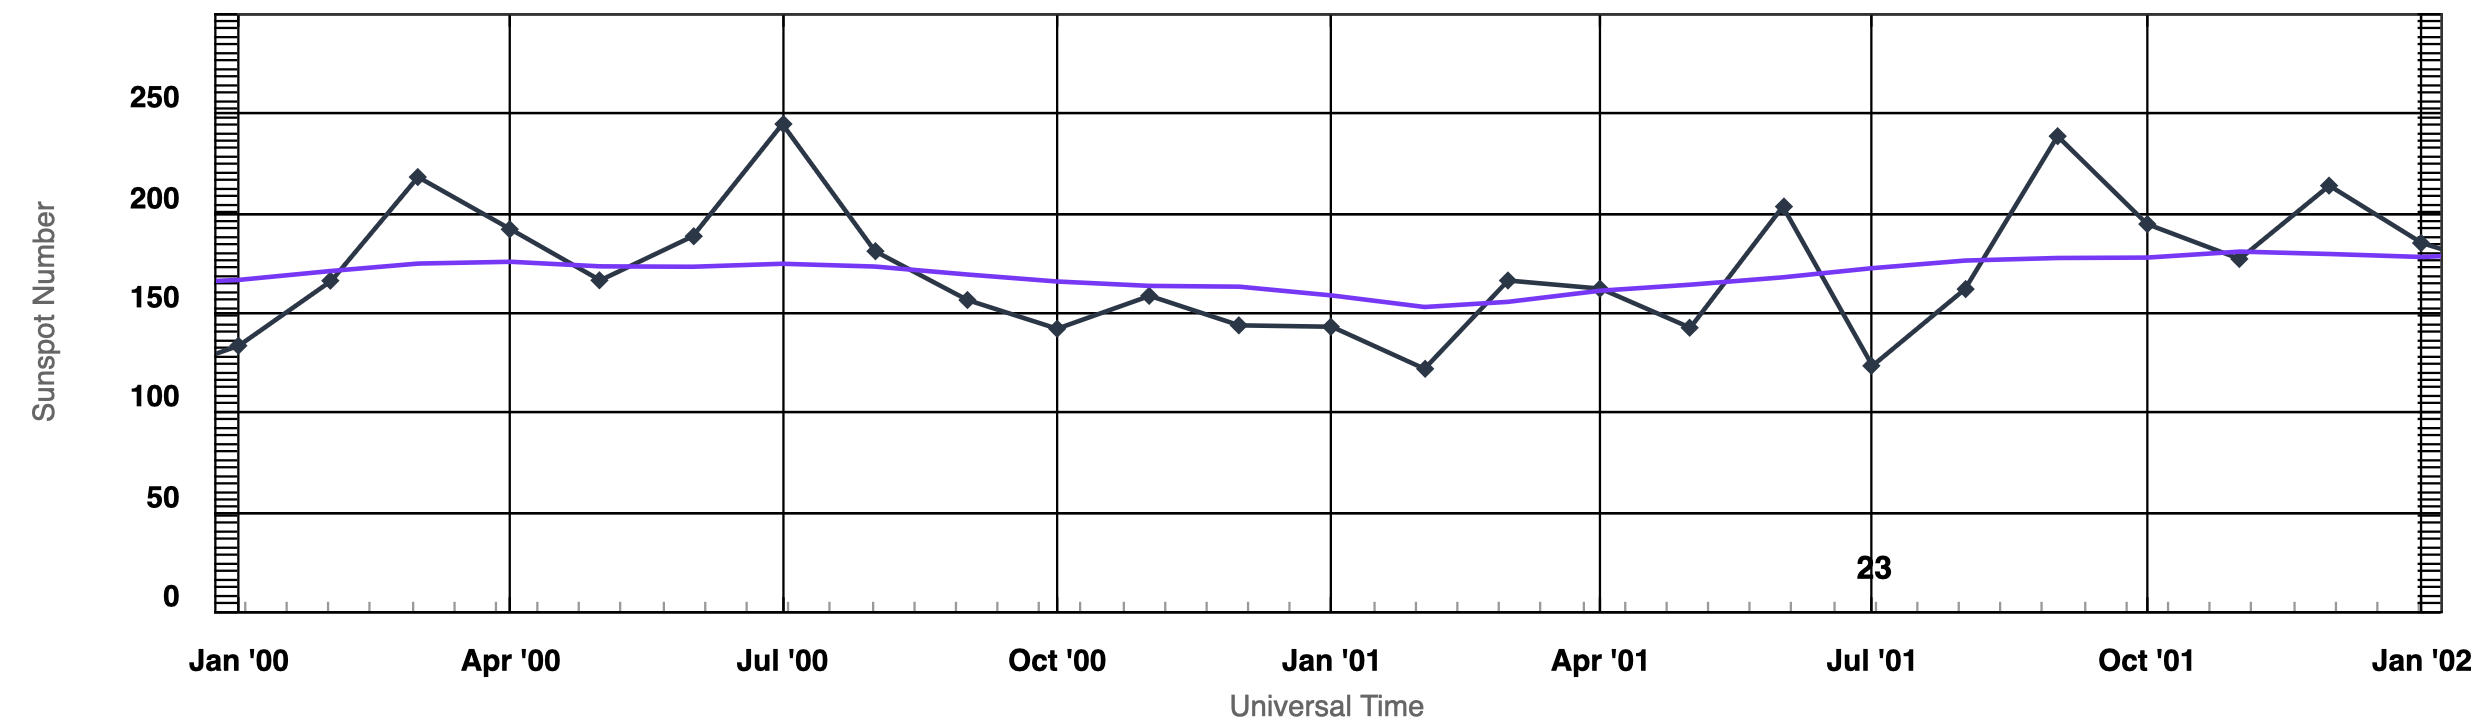
\includegraphics[scale=0.25]{figures/solar_cycle_23_maximum.png}
    \label{fig:solar_cycle_23}
    \end{figure}
\end{frame}

\begin{frame}{Processed Data}
    \begin{figure}[h]
    \centering
    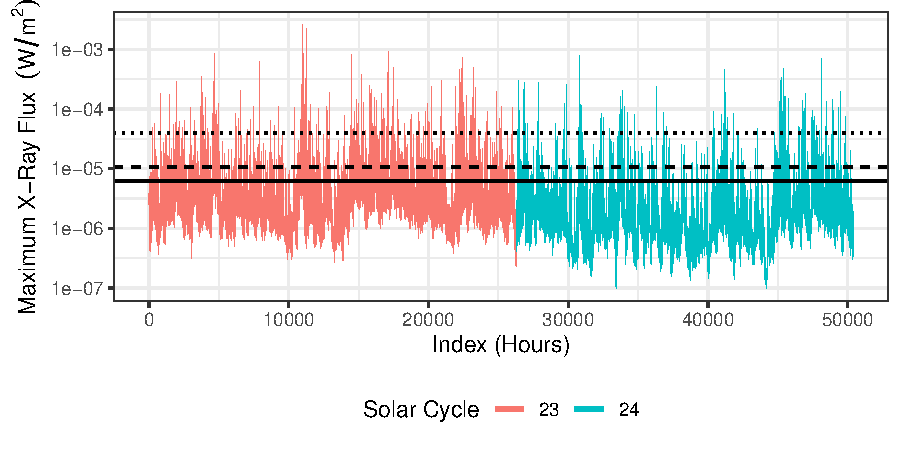
\includegraphics[width=\textwidth]{figures/goes_flux_time_series.pdf}
    \label{fig:goes_flux_time_series}
    \end{figure}
\end{frame}

\begin{frame}{Further Data Processing}
    \begin{itemize}
        \item The final time series was divided into windows of size 4,320 (the number of hours in 180 days).
        \item Consecutive windows differed in their starting times by 12 observations.
        \item Total number of windows: 3,840.
    \end{itemize}
\end{frame}

\begin{frame}{Prediction Models}
    Over each window, three models were fit, exceedances of the $p$th marginal quantile $h$ hours ahead were predicted, for
    \begin{itemize}
        \item $p \in \{0.9, 0.95, 0.99\}$
        \item $h \in \{1, \ldots, 24\}$
    \end{itemize}
    Models:
    \begin{itemize}
        \item Baseline model: at time $t$, predicts that $X_{t + h} \ge \tau \iff X_t \ge \tau$.
        \item AR(168) model: predicts using Algorithm~\ref{alg:AR_pred}.
        \item FARIMA$(0, d, 0)$ model with symmetric $\alpha$-stable ($S\alpha S$) innovations (following \cite{stanislavsky2009fari})
    \end{itemize}
\end{frame}

\begin{frame}{FARIMA Models}
    A FARIMA$(0, d, 0)$ model with $S\alpha S$ innovations is defined by
    \begin{equation}\label{eq:farima_0_d_0_mod}
        Y_t = (1 - B)^{-d}\epsilon_t, \quad t \in \Z,
    \end{equation}
    where the $\epsilon_t$'s are symmetric $\alpha$-stable. Examples of symmetric $\alpha$-stable distributions are Cauchy ($\alpha = 1$) and Gaussian ($\alpha = 2$).
    
    By Theorem 2.1 in \cite{kokoszka1995frac}, if $d$ is non-integral, $\alpha \in (1, 2)$, and $d < 1 - 1 / \alpha$, then the unique solution to \eqref{eq:farima_0_d_0_mod} is
    \begin{equation}\label{eq:farima_solution}
        Y_t = \sum_{j = 0}^{\infty} a_j\epsilon_{t - j},
    \end{equation}
    where
    \begin{equation}\label{eq:farima_causal_coefs}
        a_0 = 1, \quad a_j = \frac{\Gamma(j + d)}{\Gamma(d)\Gamma(j + 1)},
    \end{equation}
    $\Gamma$ being the gamma function.    
\end{frame}

\begin{frame}{FARIMA Models}
    \begin{itemize}
        \item For $\alpha \in (1, 2)$, a $S\alpha S$ random variable is regularly varying with tail index $\alpha$, i.e., for some $c > 0$, as $x \to \infty$, $\P(\epsilon_t > x) \sim c x^{-\alpha}$.
        \item For $d > 0$,
        \[
        a_j = \frac{\Gamma(j + d)}{\Gamma(d)\Gamma(j + 1)} \sim \frac{j^{d - 1}}{\Gamma(d)}, \ \ \ \mbox{as $j \to \infty$}
        \]
        \item If $\{Y_t\}$ were an AR(1) process, i.e., $Y_t = \phi Y_{t - 1} + \epsilon_t$ for all $t$, with $|\phi| < 1$, then
        \[
        a_j = \phi^j
        \]
        \item The slow decay of the $a_j$'s for FARIMA makes FARIMA long-range dependent.
    \end{itemize}
\end{frame}

\begin{frame}{Fitted FARIMA Models}
    \begin{figure}[!htb]
    \centering
    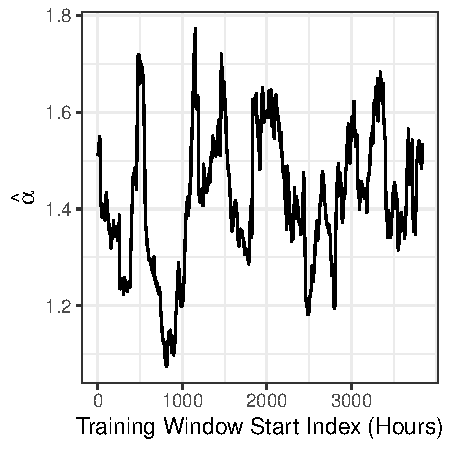
\includegraphics[width=0.32\textwidth]{farima_alpha_estims.pdf}
    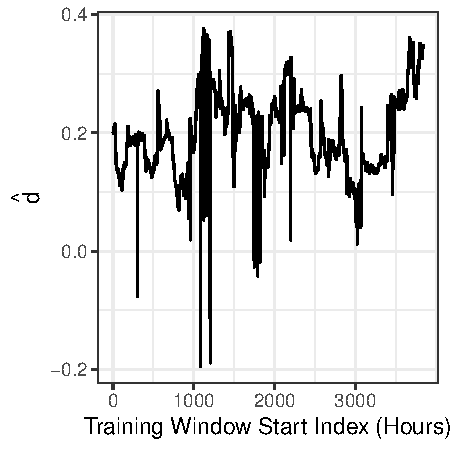
\includegraphics[width=0.32\textwidth]{farima_d_estims.pdf}
     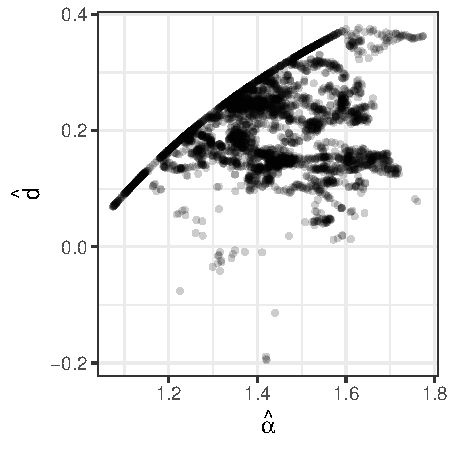
\includegraphics[width=0.32\textwidth]{farima_alpha_d_estims.pdf}
    \label{fig:farima_param_estims}
    \end{figure}
\end{frame}

\begin{frame}{Prediction Results}
    \begin{table}[ht]
    \centering
    \begin{tabular}{cc|ccc|ccc}
      \hline
      & & \multicolumn{3}{c|}{Precision} & \multicolumn{3}{c}{TSS} \\
     $h$ & $p$ & Baseline & FARIMA & AR(168) & Baseline & FARIMA & AR(168) \\
     \hline
     1 & 0.90 & {\bf 0.492} & 0.448 & 0.354 & {\bf 0.435} & 0.392 & 0.276 \\ 
       1 & 0.95 & {\bf 0.379} & 0.368 & 0.258 & {\bf 0.334} & 0.320 & 0.225 \\ 
       1 & 0.99 & {\bf 0.244} & 0.238 & 0.104 & {\bf 0.262} & {\bf 0.262} & 0.124 \\ 
       \hline
     6 & 0.90 & 0.308 & {\bf 0.339} & 0.284 & 0.256 & {\bf 0.298} & 0.215 \\ 
       6 & 0.95 & 0.189 & {\bf 0.213} & 0.150 & 0.173 & {\bf 0.198} & 0.138 \\ 
       6 & 0.99 & 0.049 & 0.119 & {\bf 0.125} & 0.040 & 0.115 & {\bf 0.162} \\ 
       \hline
    12 & 0.90 & 0.284 & {\bf 0.292} & 0.253 & 0.197 & {\bf 0.205} & 0.152 \\ 
      12 & 0.95 & {\bf 0.194} & 0.176 & 0.127 & {\bf 0.148} & 0.124 & 0.076 \\ 
      12 & 0.99 & {\bf 0.098} & 0.073 & 0.049 & {\bf 0.085} & 0.061 & 0.056 \\ 
       \hline
    18 & 0.90 & 0.270 & {\bf 0.309} & 0.253 & 0.210 & {\bf 0.256} & 0.183 \\ 
      18 & 0.95 & 0.175 & {\bf 0.197} & 0.142 & 0.154 & {\bf 0.173} & 0.117 \\ 
      18 & 0.99 & 0.049 & {\bf 0.116} & 0.067 & 0.040 & {\bf 0.115} & 0.064 \\ 
       \hline
    \end{tabular}
    \label{tab:expanded_data_analysis_results}
    \end{table}    
\end{frame}

\begin{frame}[allowframebreaks]{References}
    \printbibliography
\end{frame}

\end{document}